\header[v]{
    \headtitle{Les nuits d'une demoiselle} \label{les-nuits-d-une-demoiselle}
    %
    
    \insertComment{Chanson de Colette Renard (1963).}{}
}
\vspace{-0.5cm}
\enluminure{4}{\href{https://www.youtube.com/watch?v=mW1JxFb_7aM}{Q}}{ue} c'est bon d'être demoiselle,
\\Car le soir dans mon petit lit,
\\Quand l'étoile Vénus étincelle,
\\Quand doucement tombe la nuit,
\dualcol{
Je me fais sucer la friandise,
\\Je me fais caresser le gardon,
\\Je me fais empeser la chemise,
\\Je me fais picorer le bonbon,
\\\\... frotter la péninsule,
\\... béliner le joyau,
\\... remplir le vestibule,
\\... ramoner l'abricot,
\\\\... farcir la mottelette,
\\... couvrir le rigondin,
\\... gonfler la mouflette,
\\... donner le picotin,
\\\\... laminer l'écrevisse,
%froyer = frotter
\\... froyer le coeur fendu,
\\... tailler la pelisse,
\\... planter le mont velu,
\\\\... briquer le casse-noisettes,
\\... mamourer le bibelot,
\\... sabrer la sucette,
\\... reluire le berlingot,
\\\\... gauler la mignardise,
\\... rafraîchir le tison,
\\... grossir la cerise,
\\... nourrir le hérisson,
\\\\... chevaucher la chosette,
\\... chatouiller le bijou,
\\... bricoler la cliquette,
\\... gâter le matou,
}
Et vous me demanderez peut-être
\\Ce que je fais le jour durant?
\\Oh, cela tient en peu de lettres,
\\Le jour, je baise, tout simplement!

\begin{center}
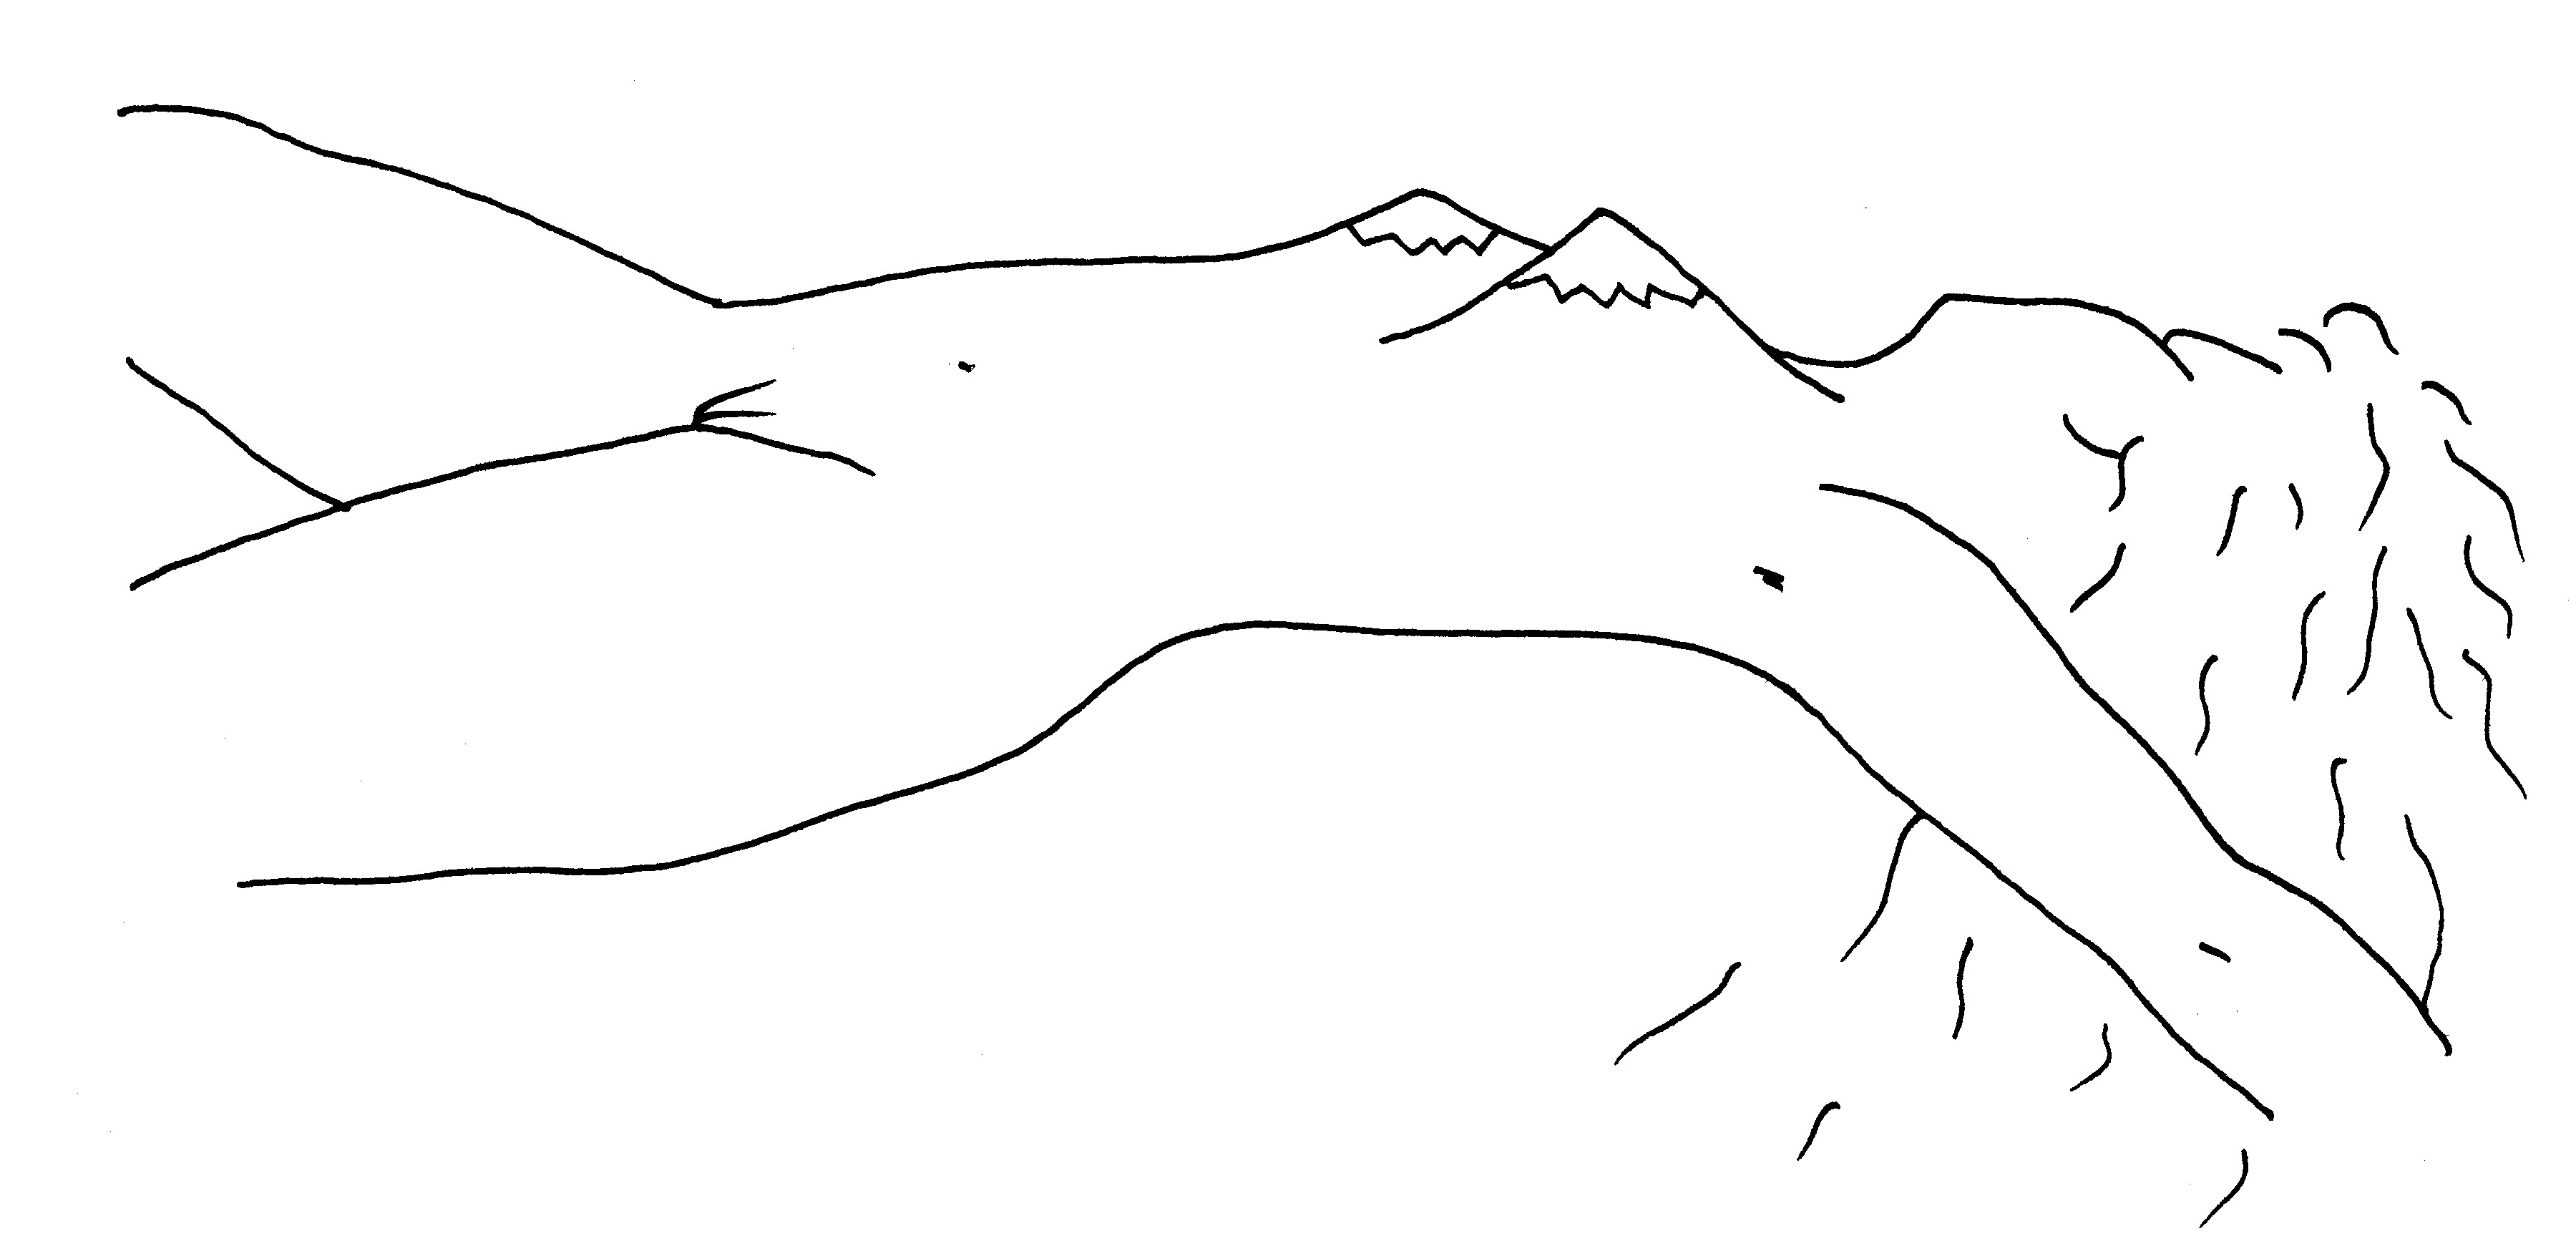
\includegraphics[width=0.7\textwidth]{images/nuit_demoiselle.jpg}
\end{center}

\breakpage